\documentclass[
  % -- opções da classe memoir --
  article,   % indica que é um artigo acadêmico
  11pt,      % tamanho da fonte
  oneside,   % para impressão apenas no recto. Oposto a twoside
  a4paper,   % tamanho do papel.
  % -- opções da classe abntex2 --
  %chapter=TITLE,        % títulos de capítulos convertidos em letras maiúsculas
  %section=TITLE,        % títulos de seções convertidos em letras maiúsculas
  %subsection=TITLE,     % títulos de subseções convertidos em letras maiúsculas
  %subsubsection=TITLE   % títulos de subsubseções convertidos em letras maiúsculas
  % -- opções do pacote babel --
  english,   % idioma adicional para hifenização
  brazil,    % o último idioma é o principal do documento
  sumario=tradicional
]{abntex2}

% ---
% PACOTES
% ---

% ---
% Pacotes fundamentais
% ---
\usepackage{lmodern}          % Usa a fonte Latin Modern
\usepackage[T1]{fontenc}      % Selecao de codigos de fonte.
\usepackage[utf8]{inputenc}   % Codificacao do documento (conversão automática dos acentos)
\usepackage{indentfirst}      % Indenta o primeiro parágrafo de cada seção.
\usepackage{nomencl}          % Lista de simbolos
\usepackage{color}            % Controle das cores
\usepackage{graphicx}         % Inclusão de gráficos
\usepackage{microtype}        % Para melhorias de justificação
\usepackage{hyperref}         % Habilita links e referências

% Termo em inglês: itálico + inglês
\newcommand{\en}[1]{\foreignlanguage{english}{\textit{#1}}}

\newcommand{\defaultFigureWidth}{0.75}

% Configuração do `minted`
\newcommand{\codigoname}{Código}
\newcommand{\listofcodigosname}{Lista de Códigos}
\newfloat[chapter]{codigo}{loc}{\codigoname}
\newlistof{listofcodigos}{loc}{\listofcodigosname}
\newlistentry{codigo}{loc}{0}
\setfloatadjustment{codigo}{\centering}
\counterwithout{codigo}{chapter}
\providecommand*{\codigoautorefname}{\codigoname}
\setfloatadjustment{codigo}{%
    \centering
    \setlength{\topsep}{0pt}%
    \setlength{\partopsep}{0pt}%
}
\usepackage[newfloat]{minted}           % Habilita blocos de códigos

% --- Header e Footer ---

\setlength{\headheight}{36pt}
\setlength{\headsep}{10pt}

\makepagestyle{meuestilo}
\makeevenhead{meuestilo}{
\includegraphics[height=1.1cm]{FCI.png}}{}{\thepage}
\makeoddhead{meuestilo}{
\includegraphics[height=1.1cm]{FCI.png}}{}{\thepage}
\makeheadrule{meuestilo}{\textwidth}{0.4pt}

\pagestyle{meuestilo}
% Para páginas "plain" (como início de capítulo/título):
\aliaspagestyle{chapter}{meuestilo}
\aliaspagestyle{plain}{meuestilo}

% Pacotes de citações
% ---
%\usepackage[brazilian,hyperpageref]{backref}   % Paginas com as citações na bibl
\usepackage[alf]{abntex2cite}   % Citações padrão ABNT
% ---

% ---
% Configurações do pacote backref
% Usado sem a opção hyperpageref de backref
%\renewcommand{\backrefpagesname}{Citado na(s) página(s):~}
% Texto padrão antes do número das páginas
%\renewcommand{\backref}{}
% Define os textos da citação
%\renewcommand*{\backrefalt}[4]{
%  \ifcase #1 %
%    Nenhuma citação no texto.%
%  \or
%    Citado na página #2.%
%  \else
%    Citado #1 vezes nas páginas #2.%
%  \fi}%
% ---

% --- Informações de dados para CAPA e FOLHA DE ROSTO ---

\titulo{Implementação de Ontologia para Gêmeos Digitais Urbanos: Um estudo de caso da Universidade Presbiteriana Mackenzie}
\def \theforeigntitle{}

\autor{Daniel Yoshio Omiya\textsuperscript{1}
  \and Gabriel Mason Guerino\textsuperscript{1}
  \and Pedro Bacic Branco\textsuperscript{1}
  \and Prof. Dr. Fabio Silva Lopes\textsuperscript{1,2} \\
  \\
  \textsuperscript{1}Faculdade de Computação e Informática (FCI) \\ Universidade Presbiteriana Mackenzie São Paulo–SP – Brasil \\
  \\ \textsuperscript{2}Programa de Pós-Graduação em Computação Aplicada \\ Universidade Presbiteriana Mackenzie São Paulo–SP – Brasil \\
  \\
  \url{{10356170,10409928,10382476}@mackenzista.com.br}
  \\
\url{fabio.lopes@mackenzie.br}}

\data{2026}
% ---

% ---
% Configurações de aparência do PDF final

% alterando o aspecto da cor azul
\definecolor{blue}{RGB}{41,5,195}

% informações do PDF
\makeatletter
\let\@fnsymbol\@arabic
\hypersetup{
  %pagebackref=true,
  %pdftitle={\@title},
  %pdfauthor={\@author},
  %pdfsubject={Modelo de artigo científico com abnTeX2},
  %pdfcreator={LaTeX with abnTeX2},
  %pdfkeywords={abnt}{latex}{abntex}{abntex2}{atigo científico},
  colorlinks=true,      % false: boxed links; true: colored links
  linkcolor=blue,       % color of internal links
  citecolor=blue,       % color of links to bibliography
  %filecolor=magenta,   % color of file links
  urlcolor=blue,
  %bookmarksdepth=4
}
\makeatother
% ---

% ---
% compila o indice
% ---
\makeindex
% ---

% ---
% Altera as margens padrões
% ---
\setlrmarginsandblock{3cm}{3cm}{*}
\setulmarginsandblock{3cm}{3cm}{*}
\checkandfixthelayout
% ---

% ---
% Espaçamentos entre linhas e parágrafos
% ---

% O tamanho do parágrafo é dado por:
\setlength{\parindent}{1.3cm}

% Controle do espaçamento entre um parágrafo e outro:
\setlength{\parskip}{0.2cm}   % tente também \onelineskip

% Espaçamento simples
\SingleSpacing

\begin{document}
\selectlanguage{brazil}

% Retira espaço extra obsoleto entre as frases.
\frenchspacing

% ----------------------------------------------------------
% ELEMENTOS PRÉ-TEXTUAIS
% ----------------------------------------------------------

%---
%
% Se desejar escrever o artigo em duas colunas, descomente a linha abaixo
% e a linha com o texto ``FIM DE ARTIGO EM DUAS COLUNAS''.
% \twocolumn[        % INICIO DE ARTIGO EM DUAS COLUNAS
%
%---

% página de titulo principal (obrigatório)
\maketitle
% titulo em outro idioma (opcional)

\begin{resumoumacoluna}
  \textit{Plataformas de Gêmeos Digitais Urbanos integram dados provenientes de múltiplos sistemas heterogêneos para suportar o monitoramento e a gestão inteligente de ambientes urbanos.
    No entanto, a ausência de um vocabulário semântico comum entre esses sistemas compromete a
    interoperabilidade e limita a capacidade de raciocínio automatizado sobre os dados coletados.
    Este trabalho propõe a modelagem e implementação de uma ontologia de domínio, alinhada aos padrões
    CityGML e SOSA/SSN, para representar entidades físicas, sensores e relações espaciais no contexto
    de um campus universitário (tomado como instância controlada de gêmeo digital).
    A pesquisa adota a metodologia \en{Design Science Research} (DSR), compreendendo a revisão dos
    padrões de referência, a modelagem da ontologia, a definição de um mecanismo de exposição, e a
    validação.
    Os resultados incluem uma ontologia capaz de responder a perguntas semânticas
    do campus, promovendo interoperabilidade entre fontes de dados diversas na plataforma de Gêmeo Digital
    da Universidade Presbiteriana Mackenzie.
  }

  \vspace{\onelineskip}

  \noindent
  \textbf{Palavras-chave}: cidades inteligentes; gêmeos digitais urbanos; ontologia; dados semânticos; CityGML; SOSA/SSN.
\end{resumoumacoluna}

\renewcommand{\resumoname}{Abstract}
\begin{resumoumacoluna}
  \begin{otherlanguage*}{english}
    \textit{Urban Digital Twin platforms integrate data from multiple heterogeneous systems to support the monitoring and intelligent management of urban environments.
      However, the absence of a common semantic vocabulary among these systems compromises
      interoperability and limits the ability to perform automated reasoning over the collected data.
      This work proposes the modeling and implementation of a domain ontology, aligned with the CityGML
      and SOSA/SSN standards, to represent physical entities, sensors, and spatial relationships within
      the context of a university campus (used as a controlled digital twin instance).
      The research adopts the Design Science Research (DSR) methodology, encompassing the review of
      reference standards, ontology modeling, the definition of an exposure mechanism, and validation.
      The results include an ontology capable of answering semantic queries about the
      campus, promoting semantic interoperability among diverse data sources within the Digital Twin platform of
      Mackenzie Presbyterian University.
    }

    \vspace{\onelineskip}

    \noindent
    \textbf{Keywords}: smart cities; urban digital twins; ontology; semantic data; CityGML; SOSA/SSN.
  \end{otherlanguage*}
\end{resumoumacoluna}

% ]          % FIM DE ARTIGO EM DUAS COLUNAS
% ---

% ----------------------------------------------------------
% ELEMENTOS TEXTUAIS
% ----------------------------------------------------------
\textual

% ----------------------------------------------------------
% Introdução
% ----------------------------------------------------------
\section{Introdução}

Segundo o relatório de Perspectiva de Urbanização Mundial da \citeonline{undesa2025wup}, as cidades
são o lar de mais de 45\% da população mundial, dobro da proporção de 1950, e projetado para chegar
a dois terços até 2050.
Esse fenômeno de crescimento acelerado das cidades eleva grandemente a complexidade de prover
infraestrutura de transporte, energia, saneamento, e governança; torna ineficiente e insuficiente
os modelos tradicionais de gestão urbana, muitas vezes com dados fragmentados em diversos sistemas
heterogêneos.
Nesse cenário, surgem as \en{Smart Cities} (Cidades Inteligentes), dotadas do uso de Internet das
Coisas (IoT), de Inteligência Artificial (IA), e da análise de quantidades massivas de dados
(\en{Big Data}), que representaram um salto no planejamento urbano, melhorando a qualidade de vida,
a eficiência da operação e dos serviços urbanos, e a tomada de decisão pública
\cite{WEIL2023104862}.

Nesse contexto, os Gêmeos Digitais Urbanos (GDU) despontam como uma tecnologia para evoluir ainda
mais a gestão e o planejamento urbano.
O Gêmeo Digital é definido como uma representação virtual de um objeto da realidade, atualizado
constantemente em um fluxo de dados bidirecional entre os mundos físico e digital.
Quando aplicado à escala urbana, torna-se uma plataforma capaz de monitorar, analisar e prever
sistemas complexos em tempo real.
Casos como o projeto \en{Virtual Singapore} e a iniciativa Helsinki 3D+ demonstram o poder deste
tipo de integração, sendo usados até mesmo para resposta a emergências
\cite{FERREBIGORRA2022103905, WEIL2023104862}.

Embora seja uma tecnologia com grande potencial, ela enfrenta uma série de desafios na sua
concepção, oriundos da fragmentação dos dados necessários em sistemas que falam dialetos
diferentes, como sensores de IoT, modelos de informação de edificações, dados geoespaciais em
padrões como CityGML, imagens de câmeras, drones e estações meteorológicas, entre outros.
Por exemplo, um sensor de IoT pode registrar a temperatura como um valor inteiro em graus Célsius,
enquanto a estação meteorológica poderia usar Fahrenheit.
Essa dificuldade de interoperabilidade é chamada de \en{semantic gap} (lacuna semântica), como
apontado por \citeonline{WEIL2023104862}.

Superar essa dificuldade requer revisar o conhecimento em comum, atribuindo um significado formal e
objetivo a cada entidade presente no domínio.
Nesse sentido, as ontologias formais apresentam-se como uma abordagem promissora
\cite{metral_ontologybased_2010}.
Elas permitem que sistemas compreendam e interoperem com dados de múltiplas origens a partir de um
vocabulário comum e de regras de inferência lógica.

O presente trabalho tem como objeto de estudo a aplicação dessas tecnologias no contexto do campus
Higienópolis da Universidade Presbiteriana Mackenzie (UPM), adotando como instância representativa
um GDU em escala reduzida.
A pesquisa é conduzida sob o paradigma da \en{Design Science Research} (DSR), que orienta o
processo de construção e avaliação de artefatos computacionais como resposta a problemas práticos
relevantes \cite{hevner_2004}, sendo a ontologia de domínio proposta o artefato central a ser
desenvolvido, avaliado e documentado.

O restante deste trabalho está organizado da seguinte forma: a Seção 2 apresenta a revisão teórica
dos fundamentos e padrões envolvidos; a Seção 3 descreve a metodologia adotada; a Seção 4 detalha a
arquitetura e a modelagem da ontologia proposta; a Seção 5 apresenta o Estudo de Caso; e a Seção 6
traz as considerações finais.

\section{Referencial Teórico}

O Gêmeo Digital é um conceito introduzido por Michael Grieves em 2003, quando ``apresentou a versão
digital de um produto físico'' \apud[p.~7]{Opoku_2021}{Gomes_2025}, e trata-se desta representação
virtual de um objeto real, atualizada continuamente através da integração entre os sistemas físico e
digital \cite{DIHAN2024e26503}.
Gêmeos Digitais aplicados à gestão urbana começaram a surgir por volta de 2018, potencializados
pelo conceito das \en{smart cities}, onde cidadãos e a administração pública cooperam em prol de
tornar a cidade mais eficiente, inteligente, sustentável, segura, inclusiva e democrática.

Os Gêmeos Digitais Urbanos (GDU) são relativamente recentes; porém, vale destacar que não são a
primeira tecnologia aplicada à geografia urbana, que, na década de 2000, já contava com o
\en{Building Information Modeling} (BIM) e o \en{Geographic Information System} (GIS), os quais são
modelagens 3D das edificações e do espaço externo.
A diferença fundamental entre estes e o GDU reside no fluxo de dados: enquanto o BIM e o GIS são
modelos estáticos, o Gêmeo Digital é dinâmico e projetado para atuar com tecnologias de IoT,
refletindo, assim, sempre informações do mundo real, como temperatura, ruído sonoro, ocupação, etc.

Contudo, ainda há um problema latente de falta de padronização e de interoperabilidade na
implementação dos GDUs, visto que poucos deles conseguem compartilhar dados com outros GDUs ou
organizações \cite{FERREBIGORRA2022103905}.
Dessa demanda, em 2008, foi desenvolvido pelo \en{Open Geospatial Consortium} (OGC) o \en{City
  Geography Markup Language} (CityGML), um padrão internacional para representar e trocar dados de
modelos 3D de cidades.
Este já é usado em regiões da Europa, sendo que todas as capitais europeias disponibilizam modelos
CityGML, bem como alguns países na Ásia e na África \cite{buildings13071758}.

O CityGML representa um grande passo na padronização da troca de informação entre sistemas de GDUs.
Todavia, segundo \citeonline[p.~103, tradução nossa]{metral_ontologybased_2010}, ``[...]
desenvolver um modelo urbano universal único é impossível; a percepção da realidade urbana é
diversa e múltipla''.
Por isso, propõe o uso de ontologias formais como ponte semântica entre diferentes modelos urbanos,
enquanto mantém o CityGML como modelo genérico para conceitos centrais compartilhados por
diferentes representações especializadas de dados urbanos.

As ontologias são definições formais de instâncias de objetos, grupos de objetos, e as relações
entre estes num domínio.
São representadas usando \en{Web Ontology Language} (OWL) e \en{Resource Description Framework}
(RDF), e, diferente de esquemas de bancos de dados, descrevem o mundo real, não a maneira como a
informação é armazenada \cite{metral_ontologybased_2010}.
O uso de ontologias num mesmo contexto (e.g., cidade ou campus universitário) pode enfrentar
desafios semânticos quando temos fontes de dados heterogêneas, como BIM, GIS, sensores de IoT, etc.
Então, sob esse olhar, a abordagem de \citeonline{metral_ontologybased_2010} mostra-se ainda mais
conveniente, dada a possibilidade de integrar estruturas de dados diversas, definindo relações de
compatibilidade semântica entre uma ontologia específica e outra \cite{SHI2023102114}.

Por fim, a ontologia \en{Sensor, Observation, Sample, and Actuator/Semantic Sensor Network}
(SOSA/SSN), proposta para sistemas de IoT, complementa o CityGML na camada de sensores.
Oriunda do trabalho em conjunto do OGC com o \en{World Wide Web Consortium} (W3C), a primeira,
SOSA, define os conceitos de sensor, observação, amostragem e atuador, enquanto a SSN a estende,
incluindo também instruções de procedimentos, propriedades observadas e sistemas de sensores
\cite{haller2019}; isso permite que dispositivos distintos, como uma câmera de segurança e um
detector de presença, observando um evento físico com dialetos diferentes, cheguem à mesma
conclusão (e.g., ``há uma pessoa no pátio'').
Assim, CityGML, SOSA/SSN e OWL/RDF formam os pilares semânticos para a modelagem do campus
Higienópolis do Instituto Presbiteriano Mackenzie, objeto central deste trabalho.

\section{Metodologia}

\subsection{Design Science Research}

Este trabalho é, quanto ao tipo, uma pesquisa aplicada, visto que busca gerar insumos para resolver
uma dificuldade real: a falta de homogeneidade nas aplicações de GDU.
Quanto à abordagem, é formal, porque o objeto central de estudo é a modelagem formal de uma
ontologia aplicada ao contexto do campus da UPM.
Em relação aos objetivos, é de natureza exploratória, pois a aplicação de ontologias OWL como
camada semântica integradora em contextos de campus universitário, como instância de GDU, ainda é
incipiente na literatura.
Por fim, quanto ao procedimento técnico, adota-se o \en{Design Science Research} (DSR).

O DSR é adotado devido ao foco em criar e avaliar um artefato para resolver um problema complexo
e/ou prático, ao passo que contribui com novos conhecimentos \cite{hevner_2004}.
Com isso, este trabalho deve gerar um artefato de modelo, o qual é a ontologia para representar
formalmente as entidades presentes no campus, de maneira alinhada aos padrões CityGML e SOSA/SSN.
Portanto, o conhecimento científico emerge do processo de construção, refinamento e validação do
próprio artefato frente à problemática envolvida.

A avaliação do artefato produzido tem como critério permitir uma maneira de navegar nas ontologias
estudadas e, usando motores como o \en{SPARQL Protocol and RDF Query Language} (SPARQL),
responder a consultas semânticas simples, como: ``quais prédios estão paralelos à Rua da
Consolação?''; ``quais espécies de árvores estão presentes no Bosque da FAU?''; ou, ainda, ``quais
sensores observam a entrada do prédio 31?''.

\subsection{Procedimentos}

O desenvolvimento do trabalho foi organizado em etapas, abrangendo a identificação das entidades
relevantes do campus, a estruturação dos dados geográficos, a modelagem semântica, a preparação da
infraestrutura de armazenamento e o desenvolvimento de uma camada de visualização.

Inicialmente, foram identificadas entidades presentes no campus que poderiam ser representadas na
estrutura proposta, com destaque para edificações e elementos associados à infraestrutura
universitária.
Para as edificações, foram organizadas informações como o número do prédio, o identificador proveniente
do GeoSampa -- portal da Prefeitura do Município de São Paulo --, o nome da edificação, as coordenadas dos vértices de seu contorno e os valores de altitude
da base e do topo.
Os vértices foram organizados conforme os contornos externos das edificações e, quando existiam,
também foram considerados os contornos internos correspondentes a aberturas ou áreas vazadas.
As altitudes da base e do topo foram utilizadas para estabelecer a dimensão vertical dos prédios,
possibilitando a construção de representações tridimensionais simplificadas.

Para a representação das edificações, foi adotado o nível de detalhe \en{Level of Detail} (LoD) 1 do CityGML.
Nesse nível, os edifícios são representados por volumes tridimensionais simplificados, compostos
por superfícies que representam a cobertura, a base e as paredes laterais.
A partir dos vértices dos contornos, foram construídos polígonos fechados e superfícies verticais,
conectando as coordenadas correspondentes às altitudes da base e do topo.
Esse procedimento permitiu transformar tabelas de coordenadas em modelos
tridimensionais das edificações, que podem ser lidos já em \en{softwares} tradicionais de CityGML, como visto na Figura~\ref{fig:buildings}.

\begin{figure}[htbp]
    \centering
    \caption{Visualização do CityGML gerado na ferramenta da Innerscene}
    \label{fig:buildings}
    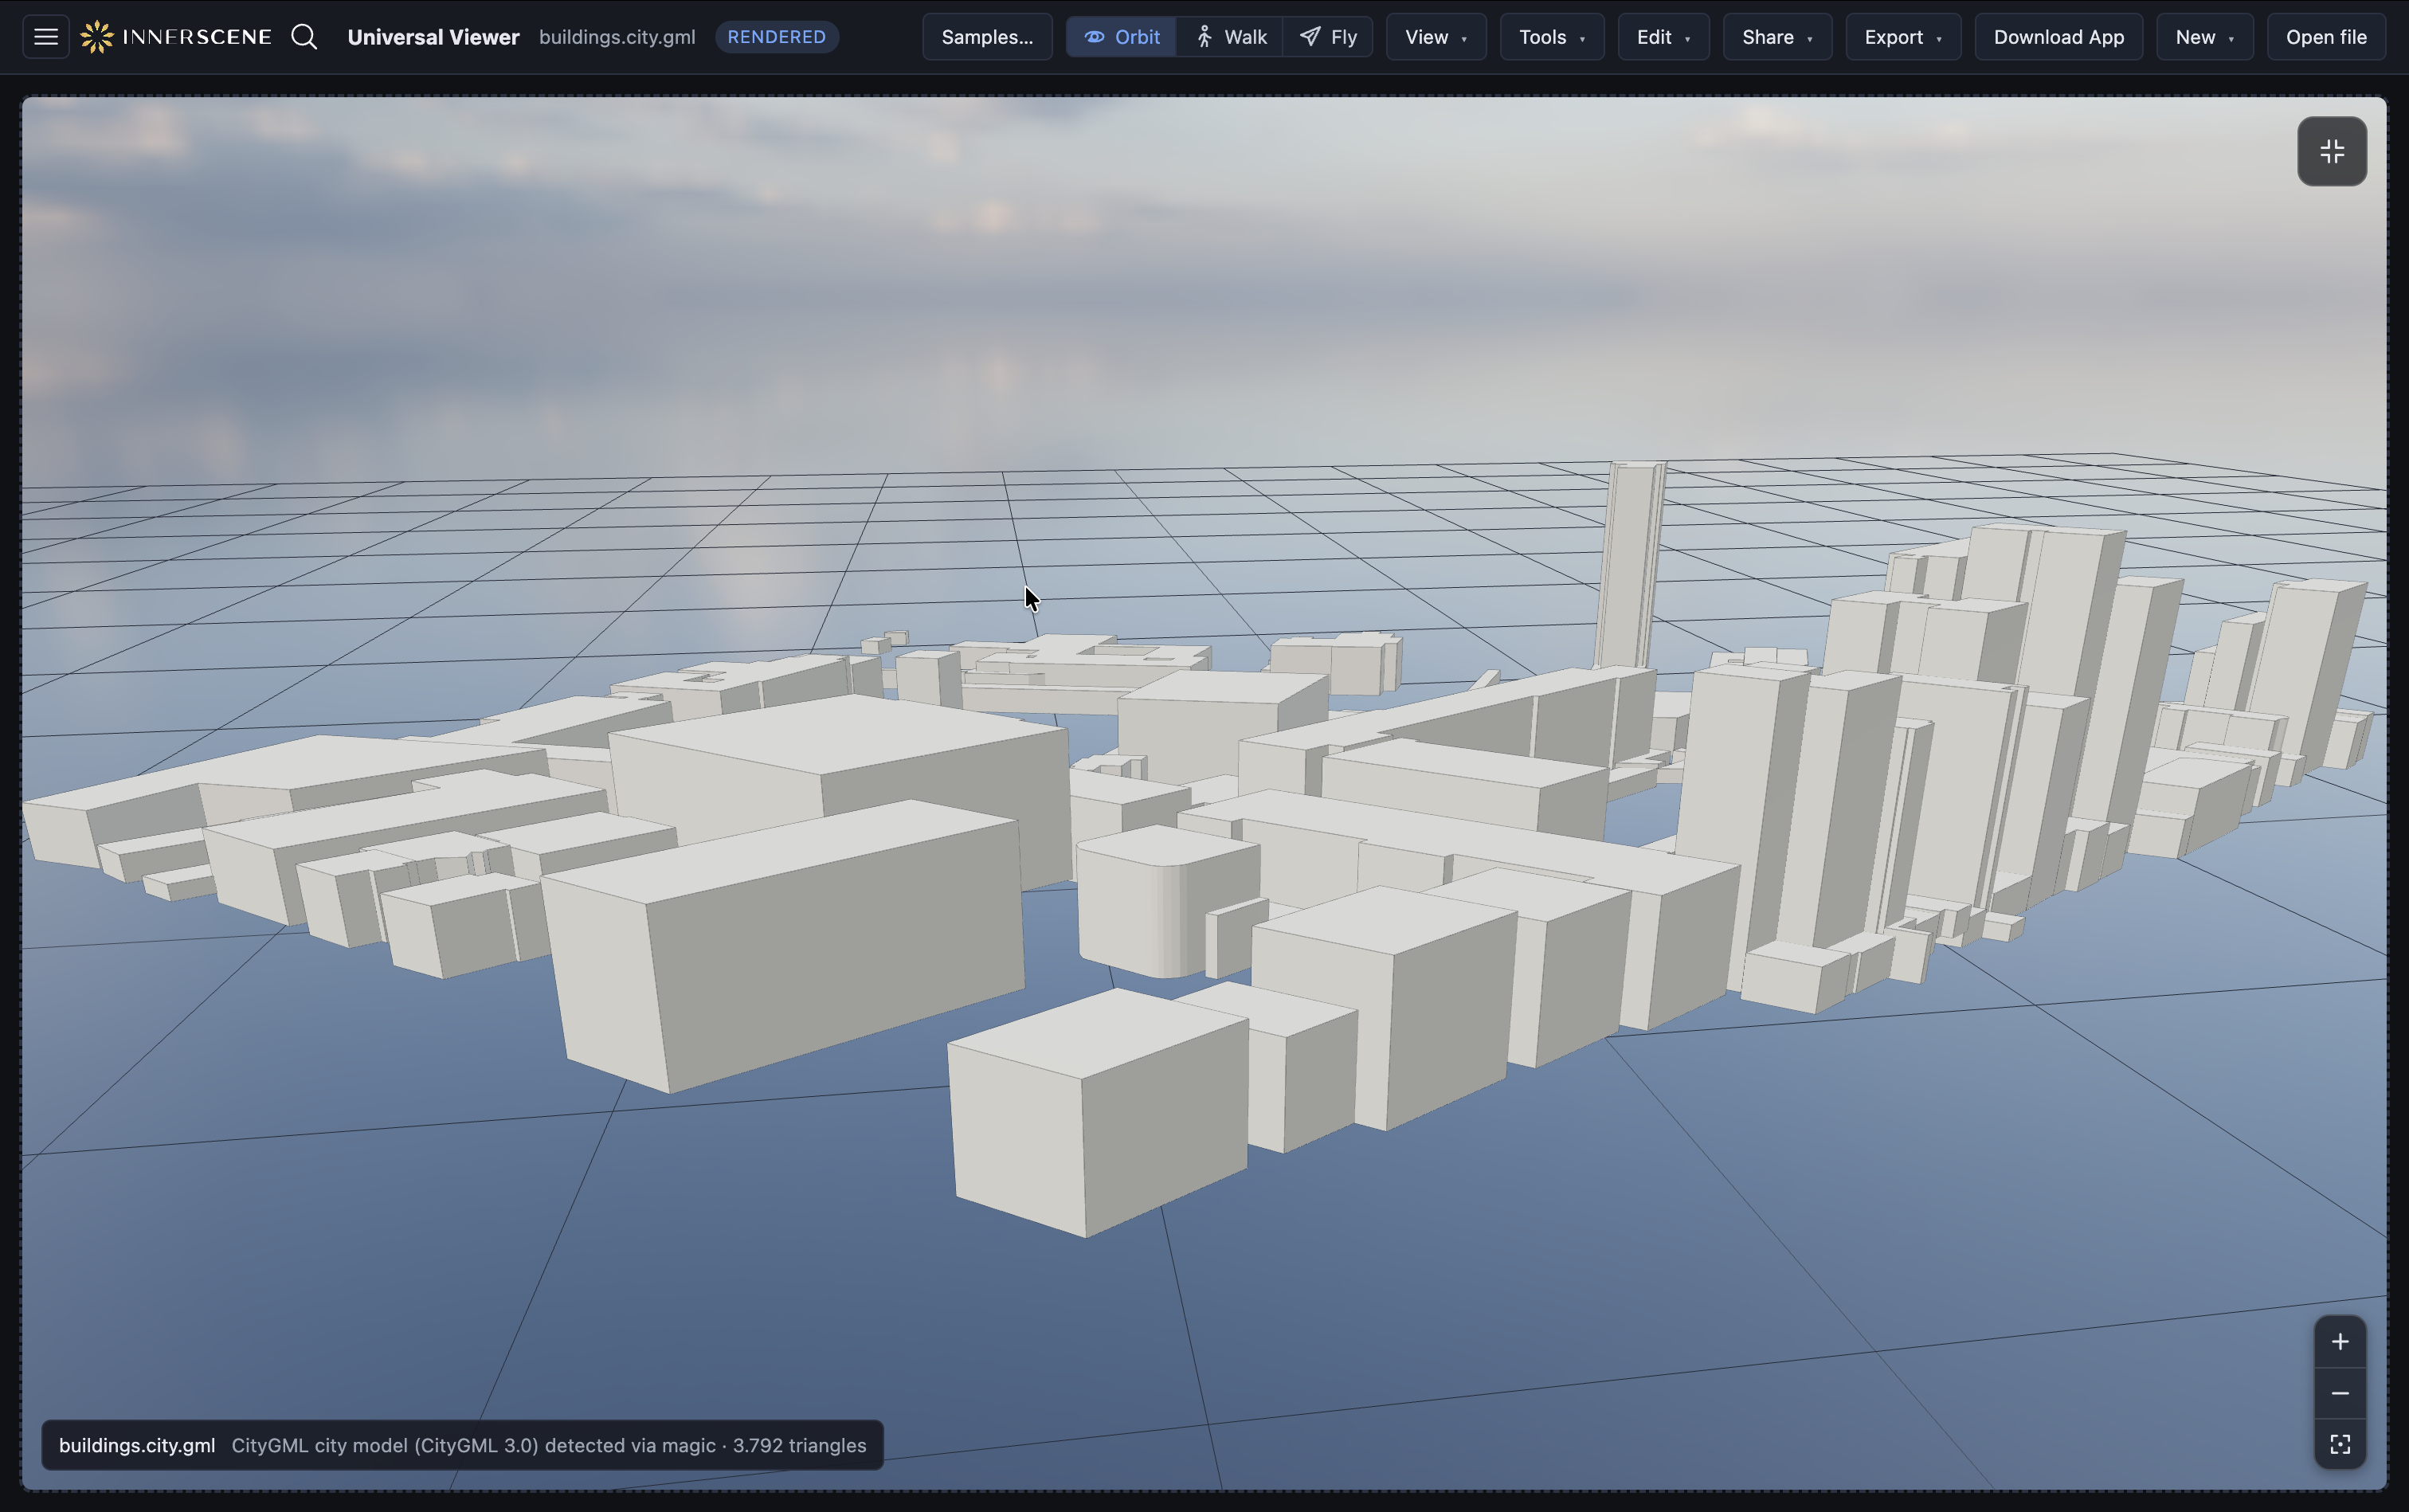
\includegraphics[width=\defaultFigureWidth\linewidth]{assets/buildings-gml.png}
    \fonte{Autoria própria.}
\end{figure}

Também foram incluídas informações descritivas dos prédios, como nomes e números internos usados para se localizar no campus,
de modo que cada geometria pudesse ser associada à respectiva entidade.
Dessa forma, os modelos não representam apenas volumes geométricos, mas também possuem informações
que permitem sua identificação e posterior relacionamento com outros dados.

Para a persistência dos modelos tridimensionais, foi configurado um ambiente utilizando Docker,
PostgreSQL com PostGIS e o 3D City Database (3DCityDB).
O 3DCityDB foi escolhido por oferecer uma estrutura de banco de dados específica para o
armazenamento e gerenciamento de modelos urbanos no padrão CityGML.
Dessa maneira, a proposta utiliza as tabelas nativas do banco, como as relacionadas aos objetos
urbanos, edificações e geometrias, evitando a criação de estruturas próprias quando já existem
estruturas equivalentes no modelo do 3DCityDB.

\begin{figure}[htbp]
    \centering
    \caption{Informações de \en{features} importadas para o 3DCityDB}
    \label{fig:citytool_info}
    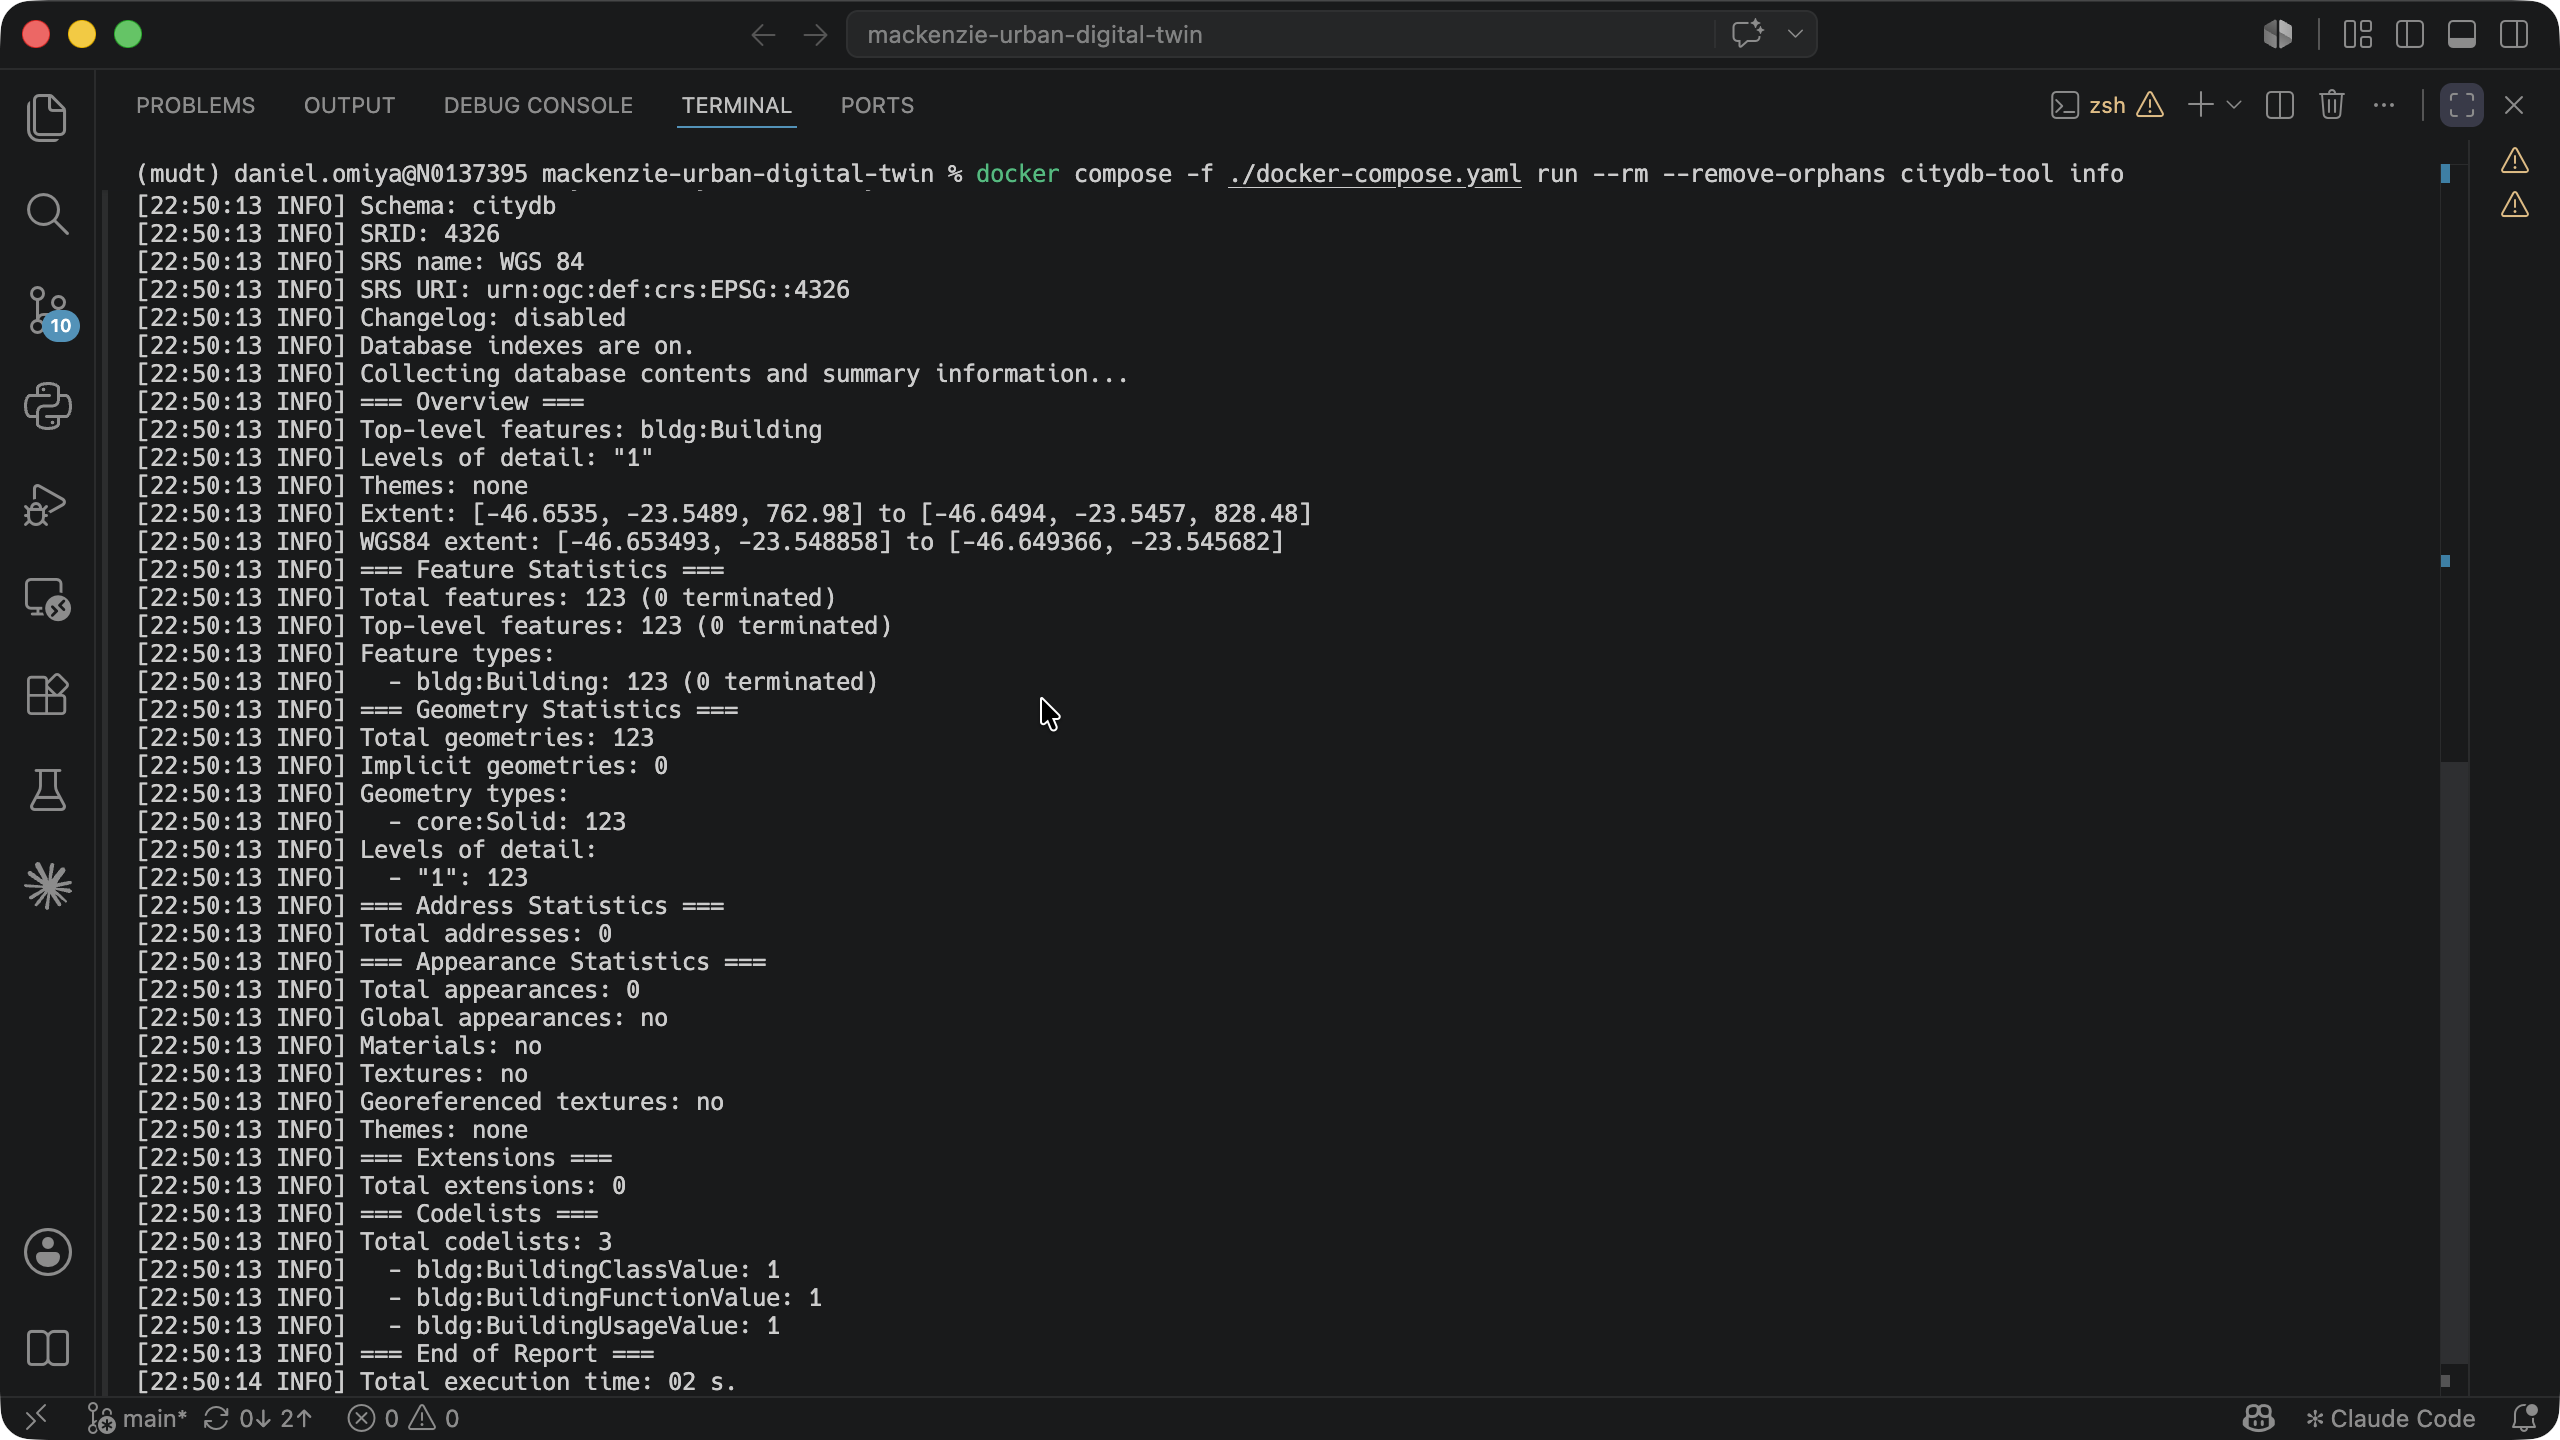
\includegraphics[width=\defaultFigureWidth\linewidth]{assets/city-tool-info.png}
    \fonte{Autoria própria.}
\end{figure}

Esses procedimentos permitiram compreender a relação entre os arquivos CityGML, o sistema de
referência espacial, o PostgreSQL e as ferramentas responsáveis pela importação e exportação dos
modelos. Por fim, foi desenvolvida uma breve página para a apresentação dos resultados, como visto na Figura~\ref{fig:cesium_1}. Nessa mesma visualização, é possível obter os detalhes de uma entidade \texttt{bldg:Building} ao clicar no polígono correspondente, como se vê na Figura~\ref{fig:cesium_2}.

\begin{figure}[htbp]
    \centering
    \caption{Visão geral gerada do campus}
    \label{fig:cesium_1}
    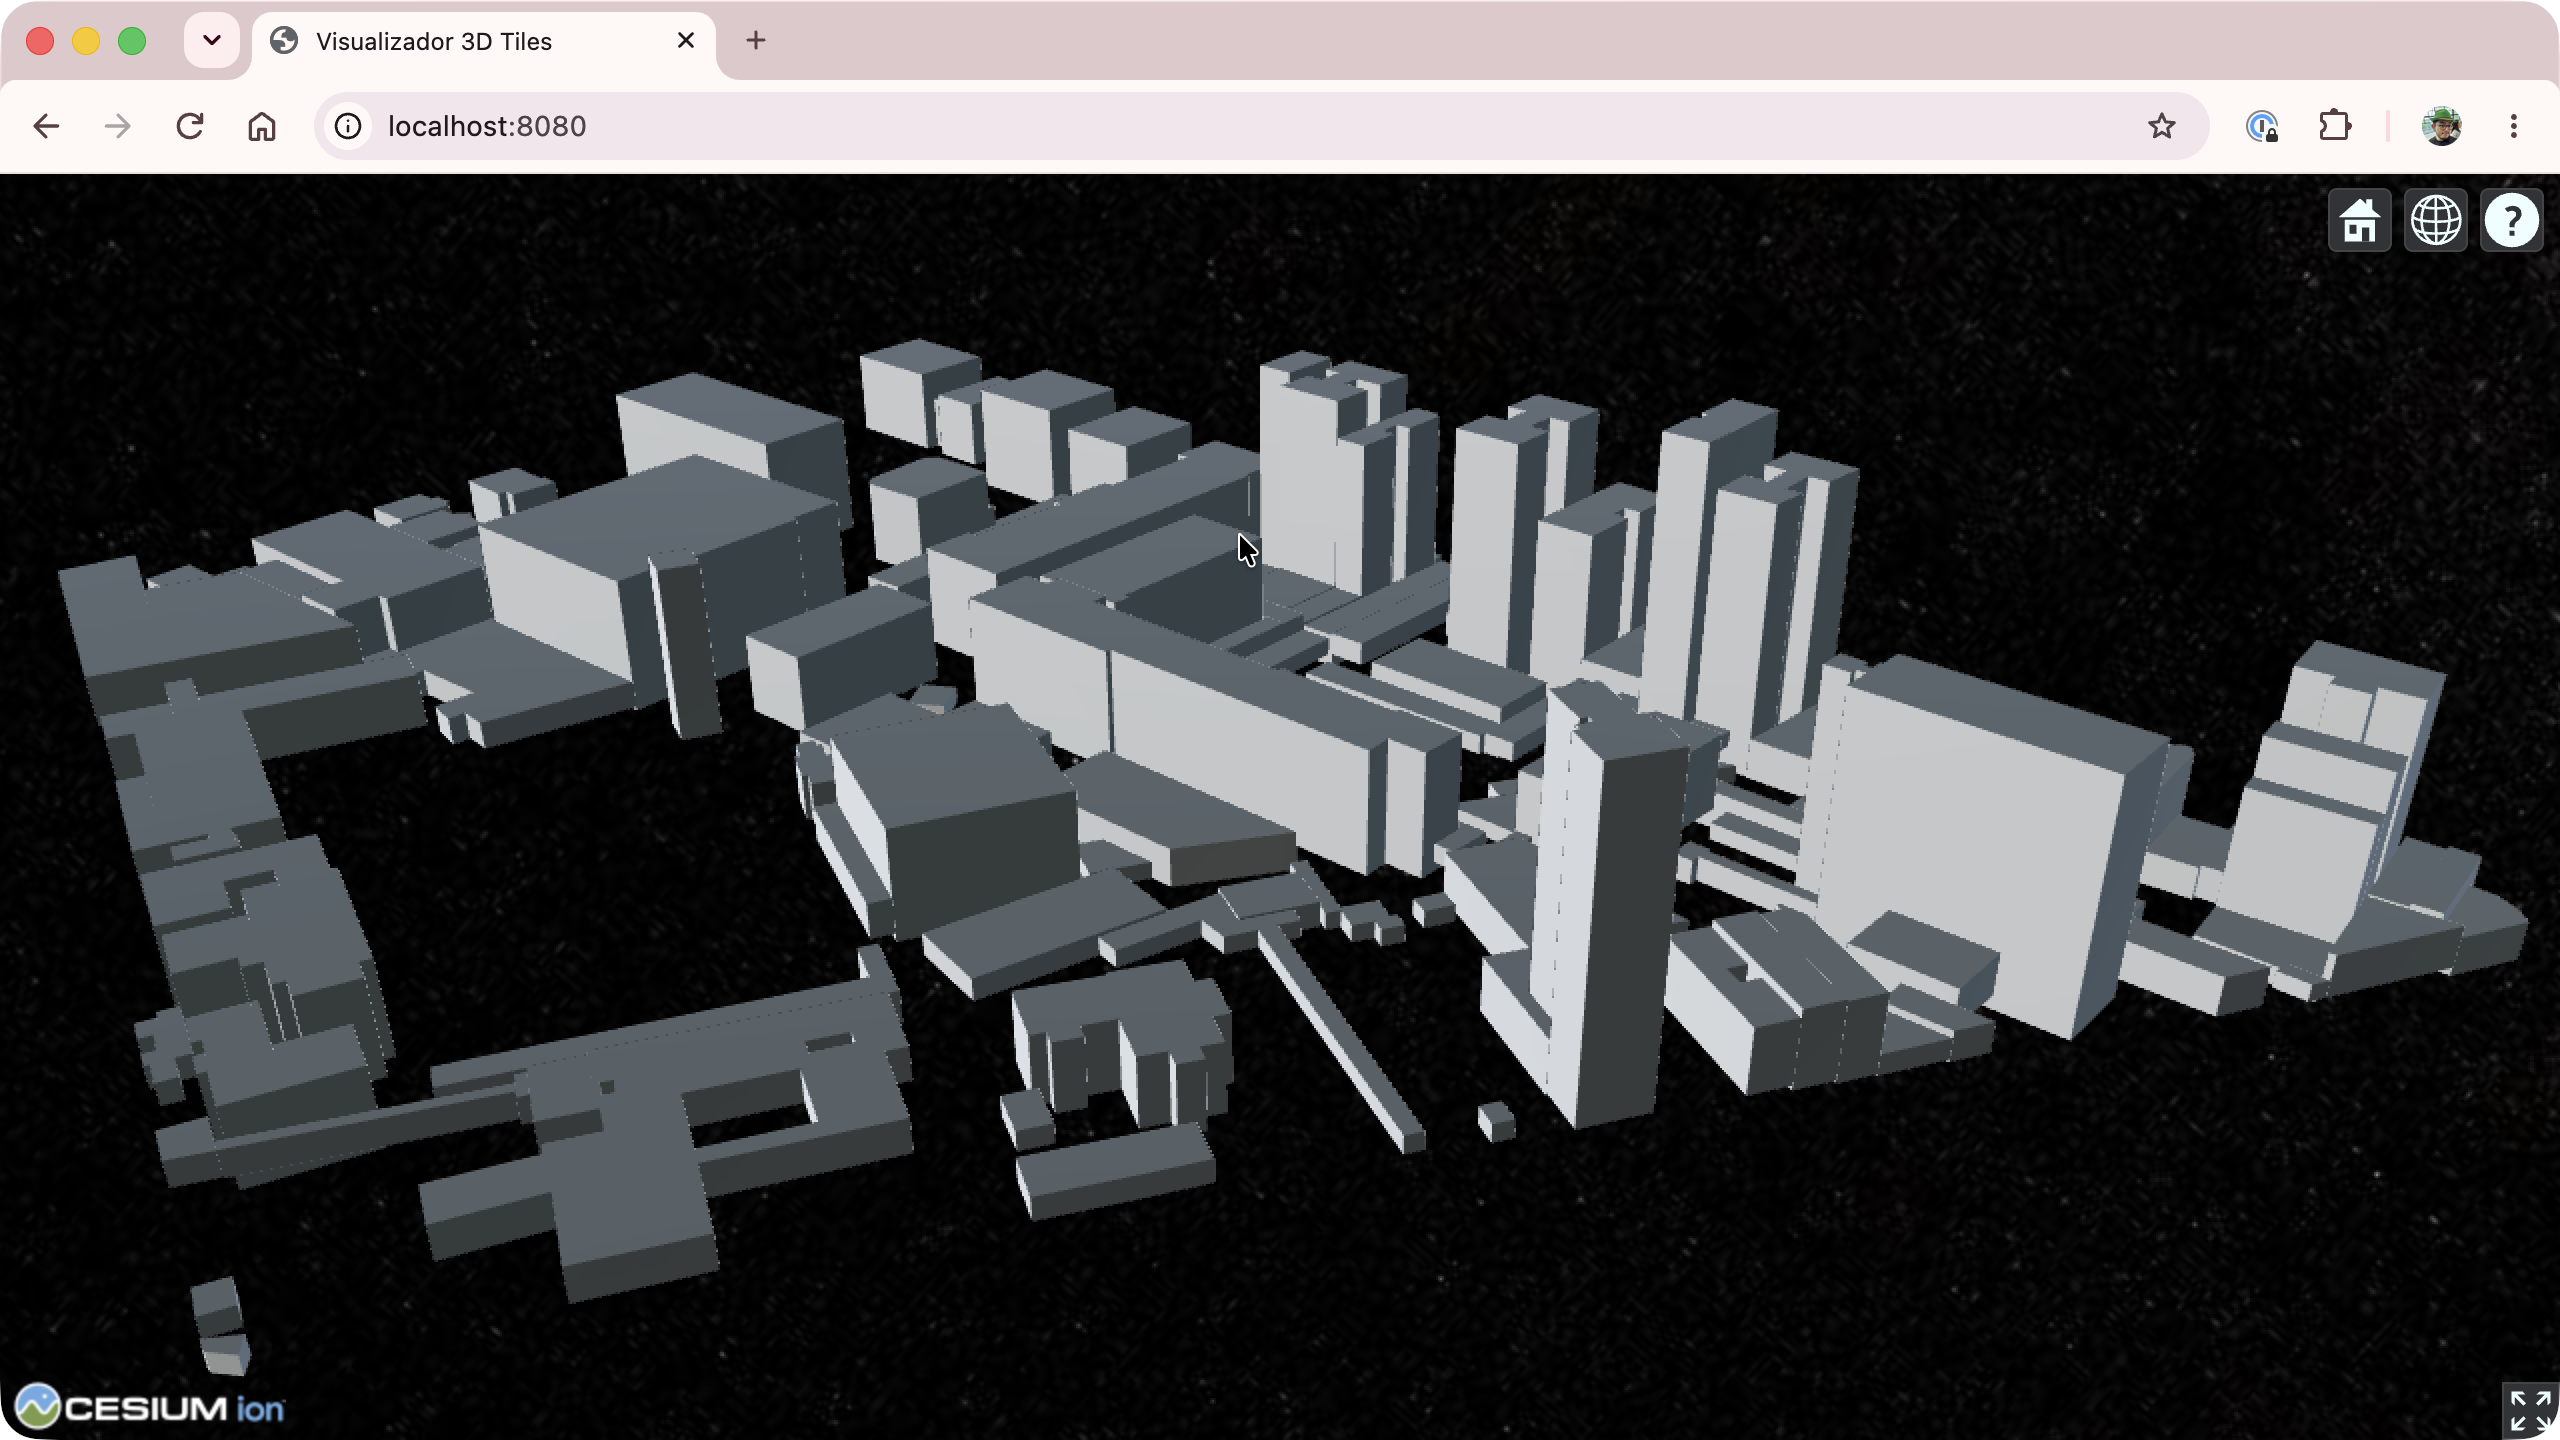
\includegraphics[width=\defaultFigureWidth\linewidth]{assets/cesium-overview.png}
    \fonte{Autoria própria.}
\end{figure}

\begin{figure}[htbp]
    \centering
    \caption{Detalhamento de uma edificação específica}
    \label{fig:cesium_2}
    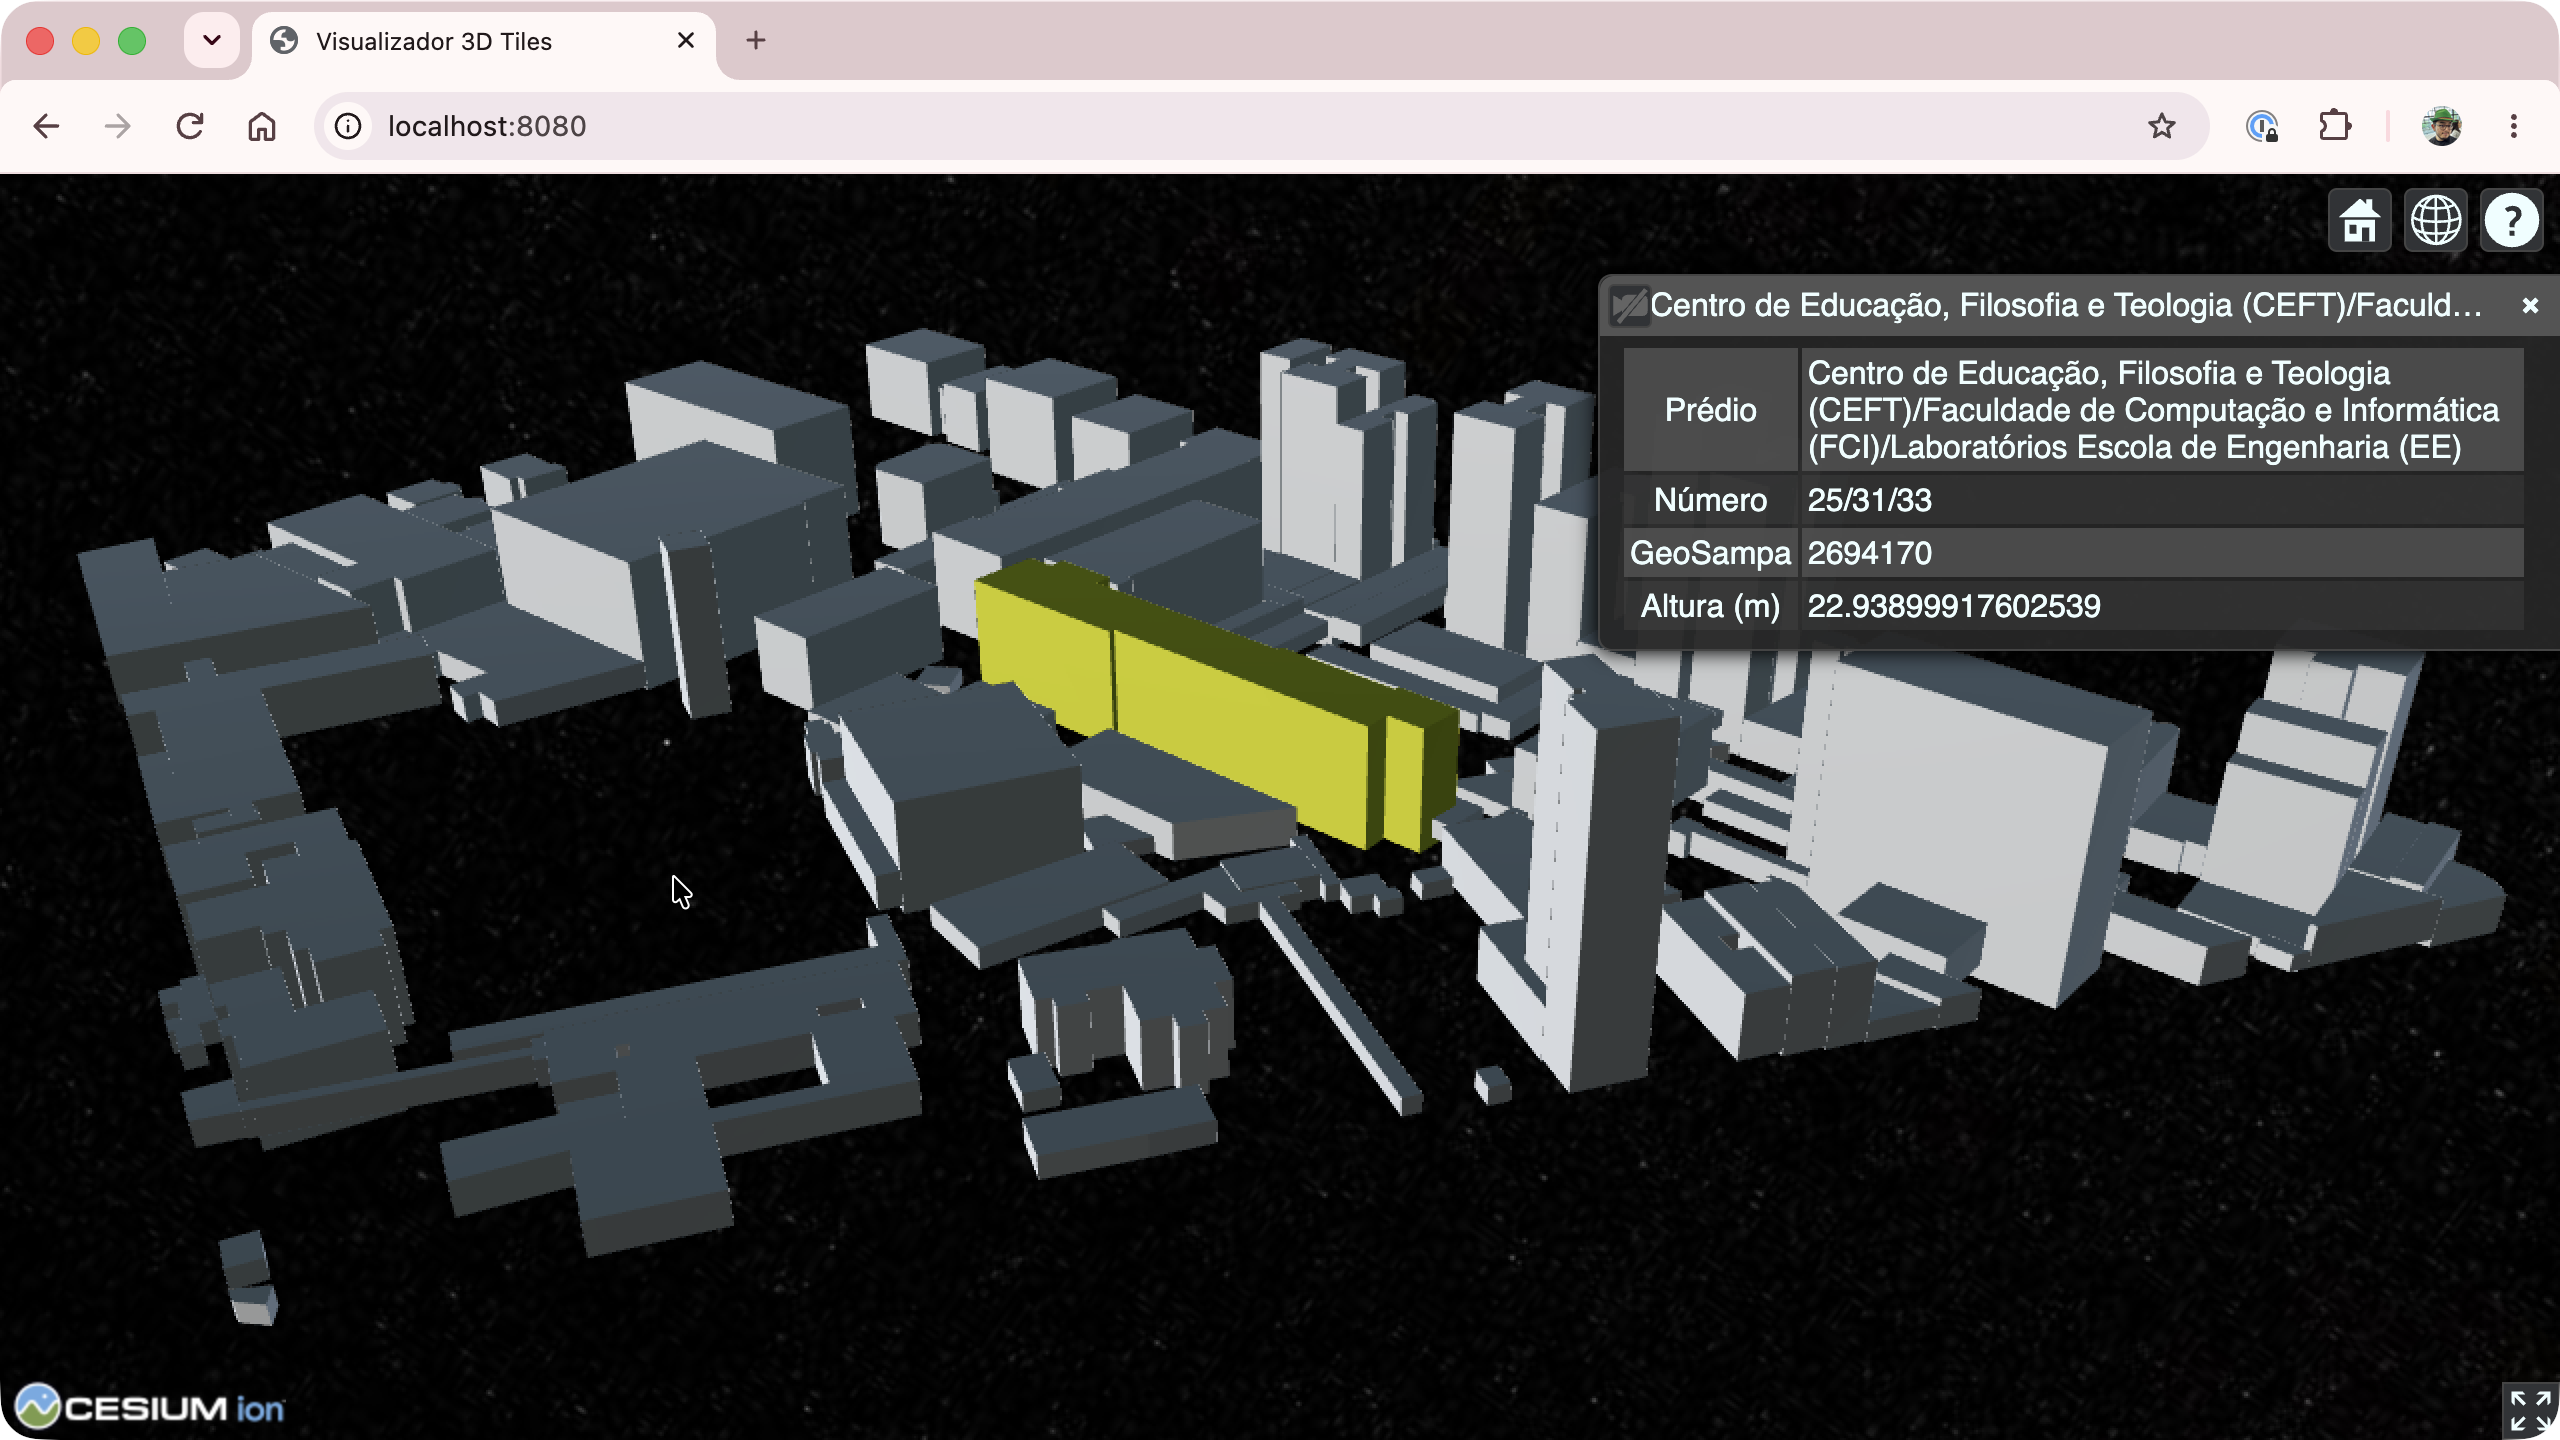
\includegraphics[width=\defaultFigureWidth\linewidth]{assets/cesium-details.png}
    \fonte{Autoria própria.}
\end{figure}

\subsection{Estratégia de Validação}

A validação do artefato foi realizada por meio de verificações relacionadas à consistência da
modelagem semântica, à representação geométrica das edificações e à capacidade de armazenamento e
consulta das informações.

Em relação aos modelos tridimensionais, foram avaliados os arquivos CityGML gerados, considerando a
identificação das edificações, a preservação dos vértices originais, a correta utilização das
altitudes da base e do topo e a construção das superfícies que compõem os volumes tridimensionais.
Também foi verificada a conformidade dos arquivos com o esquema oficial do CityGML, bem como
sua possibilidade de importação pelo 3DCityDB \en{Importer}/\en{Exporter}.

No ambiente de banco de dados, foi verificado se os modelos importados são armazenados
corretamente nas tabelas nativas do 3DCityDB e se suas informações podem ser recuperadas por meio
de consultas SQL.
Essa etapa permitiu avaliar a preservação dos identificadores, das características descritivas e
das geometrias das edificações após a importação.

A avaliação também considerou a possibilidade de visualizar diferentes edificações
simultaneamente em ferramentas de geoprocessamento ou visualização tridimensional, permitindo
observar suas posições relativas e representações espaciais dentro do campus universitário.

Além dessas questões, pretende-se verificar a possibilidade de relacionar os identificadores
utilizados na ontologia aos identificadores dos objetos armazenados no 3DCityDB, permitindo que uma
entidade seja localizada semanticamente e tenha suas características geométricas recuperadas no
banco de dados.

Dessa forma, a estratégia de validação busca verificar se o artefato atende ao objetivo de integrar
informações semânticas, geométricas e descritivas, oferecendo uma estrutura que permita
representar, armazenar, consultar e visualizar os elementos presentes no campus da Universidade
Presbiteriana Mackenzie.

\section{Arquitetura e a Modelagem da Ontologia}

\subsection{CityGML}

O CityGML é um padrão internacional, criado pelo OGC, para representar cidades em três dimensões.
Neste trabalho, ele serve como a base para descrever os elementos físicos do campus.
As edificações foram modeladas de forma simplificada: cada prédio é representado como um bloco,
construído a partir do seu contorno no mapa e esticado do chão até a altura do telhado.
Essa representação usa apenas dados disponíveis para todo o campus e é suficiente para responder às
consultas espaciais previstas na validação.

Cada edificação carrega informações como o seu identificador no GeoSampa, a sua altura, a indicação
de como essa altura foi obtida e, quando existem, o número e o nome do prédio no campus.
Os blocos foram gerados inicialmente em um formato mais simples de produzir programaticamente, o
CityJSON, e depois convertidos para CityGML com a ferramenta \texttt{citygml-tools}.
Em seguida, o modelo foi carregado no 3DCityDB, um banco de dados voltado a modelos 3D de cidades,
que armazena os blocos e seus atributos e serve de base para a construção da ontologia, descrita
nas próximas seções.

\subsection{3DCityDB}

O 3DCityDB é um banco de dados de código aberto criado para armazenar, organizar e consultar
modelos tridimensionais de cidades no formato CityGML.
Ele funciona sobre o PostgreSQL, um banco de dados amplamente utilizado, com a extensão PostGIS,
que adiciona a capacidade de trabalhar com informações geográficas, como posições, contornos e
distâncias.

Neste trabalho, o 3DCityDB cumpre o papel de repositório central dos dados do campus.
Os blocos tridimensionais das edificações, com seus atributos (identificador no GeoSampa, altura,
número e nome do prédio), foram carregados no banco a partir do arquivo CityGML, o que permite
guardar toda a informação em um único lugar e consultá-la de forma organizada.
Como o banco entende a geografia dos dados, também é possível fazer perguntas espaciais, como quais
prédios estão próximos de uma determinada rua ou quais estão em uma determinada área.

A escolha do 3DCityDB se justifica por ele seguir o mesmo padrão adotado para representar o campus,
o CityGML, sem exigir que os dados sejam convertidos para outro formato.
Assim, ele funciona como uma ponte entre o modelo 3D do campus e a ontologia proposta, que organiza
esse conteúdo a partir de um vocabulário comum e é detalhada nas próximas seções.

\subsection{Consultas Semânticas}

A partir do desenvolvimento dos dados no padrão do CityGML, que é uma taxonomia estrutural (ou
seja, é apenas um esquema de dados, não propriamente uma ontologia), podemos estendê-lo
importando-o para uma ontologia própria do domínio trabalhado e incluindo axiomas lógicos que guiam
a organização do campus universitário.
Assim, enriquecendo e dando valor semântico aos dados, o que ajuda encontrar se há contradições
lógicas na validação destes.

Este trabalho limitou-se à modelagem do campus em CityGML; porém, foi considerada a tecnologia
Apache Jena, um \en{framework} de código aberto que inclui componentes para, a partir de consultas
SPARQL, consultar bases de dados relacionais, como o 3DCityDB.
Neste modelo, cada entidade construída para o CityGML torna-se uma tripla RDF (\en{Resource Description Framework}, em tradução livre "estrutura de descrição de recursos"), que possui o formato $Sujeito \rightarrow Predicado \rightarrow Objeto$, por exemplo:

\begin{codigo}[htbp]
  \caption{Exemplo com triplas RDF}
  \label{cod:rdf_example}
  \begin{minted}[frame=single, fontsize=\footnotesize]{turtle}
mack:predio_31 a bdlg:Building ;
    bldg:hasBuildingRoom mack:sala_31_304 .

mack:sala_31_304 a bldg:BuildingRoom ;
    bldg:function "Apple Developer Academy" ;
    bldg:usage "Laboratório de máquinas Apple Mac" ;
    bldg:roomHeight "3.0"^^xsd:double .
  \end{minted}
  \fonte{Autoria própria.}
\end{codigo}

\section{Estudo de Caso}

O objetivo do estudo é verificar, de maneira prática, a aplicabilidade do padrão CityGML,
estendido, quando necessário, por meio de ontologias complementares, como a ontologia SSN/SOSA para
dados de sensores e a BIM para modelagem em microescala (enquanto o CityGML preocupa-se na escala
urbana).

Para este trabalho, o escopo limita-se ao campus universitário da Universidade Presbiteriana
Mackenzie, localizado na região central do município de São Paulo.
Trata-se de um espaço controlado, com uma série de edificações de usos e épocas diferentes,
múltiplos pontos de acesso para pedestres e para automóveis (portarias), e uma circulação diária de
milhares de pessoas, o que o torna um candidato ideal de GDU.

Foram usadas duas classes de entidades físicas do CityGML, a saber:

\begin{itemize}
  \item \textbf{Edificações}: os prédios do campus, identificados pelo número interno (e.g., Prédio~31) e pelo identificador do GeoSampa.
  \item \textbf{Portarias}: os pontos de acesso ao campus, que conectam o espaço interno ao sistema viário do entorno.
\end{itemize}

Outros objetos como árvores, mobiliário urbano, ambientes internos e dados de sensores foram
excluídos do escopo devido à disponibilidade imediata destes dados ser restrita durante o período
do trabalho; assim, escolhemos o LoD~1, que representa apenas o volume externo das edificações.

Os contornos das edificações foram obtidos do GeoSampa, portal de dados geoespaciais da Prefeitura
de São Paulo, nas camadas MDT (modelo digital de terreno) e MDS (modelo digital de superfície),
além do \en{dataset} de edificação com os identificadores utilizados pela própria prefeitura.
Por simplicidade, os dados foram recortados para conter a quadra da universidade em sua totalidade,
incluindo prédios externos além do campus.
Esses contornos e identificadores da prefeitura em mãos, mapeamos manualmente cada um para sua
designação interna de Prédio~N.

As localizações das portarias foram fornecidas pelo professor orientador em formato KML
(\en{Keyhole Markup Language}, ou ``Linguagem de Marcação Keyhole'' em tradução nossa; é um padrão
internacional adotado pelo OGC e usado por ferramentas como o Google Maps) contendo os marcadores
pontuais e respectivos nomes.

O KML utiliza coordenadas geográficas em WGS-84 (EPSG:4326), enquanto os dados do GeoSampa são
distribuídos em SIRGAS~2000/UTM~23S (EPSG:31983).
Para facilitar a integração com outras ferramentas já estabelecidas, optamos por reprojetar e
normalizar todos em WGS-84 (EPSG:4326), que é o sistema de referência padrão usado globalmente para
cartografia e navegação por satélite, incluindo o GPS.
A unificação do CRS (\en{Coordinate Reference System}, ``Sistema de Referência de Coordenadas'' em
tradução nossa) antes da geração dos modelos é necessária para que as consultas de distância
retornem valores corretos.

O ambiente de persistência foi instanciado em contêineres Docker com PostgreSQL, PostGIS e
3DCityDB, configurado com o WGS-84 (EPSG:4326).
O arquivo CityGML foi importado com a ferramenta \textit{citydb-tool} e permitiu responder a
perguntas simples a partir de consultas SQL, embora esta não possua, propriamente, o mesmo valor
semântico que uma ontologia é capaz de entregar.

Por fim, o \en{pipeline} desenvolvido neste estudo com dados públicos municipais e complementado
por informações institucionais mostrou-se suficiente para produzir um modelo LoD~1 padronizado do
campus, armazenado em uma estrutura reconhecida internacionalmente e consultável espacialmente.
O identificador GeoSampa, preservado em todas as etapas, funciona como uma chave estável para
integrar futuras fontes de dados às mesmas entidades.
Limitações conhecidas são: o LoD~1 não detalha telhados ou ambientes internos, o que enriqueceria
mais a possibilidade de análises; a associação entre dados do GeoSampa e prédios do campus foi
feita manualmente e, portanto, é sujeita a erro humano; e a ausência de dados de sensores impede,
por ora, a representação do aspecto dinâmico que distingue um Gêmeo Digital de um modelo 3D
estático.

\section{Considerações Finais}

O desenvolvimento deste trabalho permitiu explorar a aplicação de tecnologias de modelagem
tridimensional, bancos de dados geográficos e ontologias semânticas na organização das informações
do campus da Universidade Presbiteriana Mackenzie.
A partir da utilização de padrões como CityGML e OWL, foi possível estruturar uma proposta de
arquitetura voltada à integração de informações geométricas, descritivas e semânticas, contribuindo
para o desenvolvimento de uma abordagem de Gestão de Dados Urbanos.

Durante o desenvolvimento, foi possível compreender a importância da padronização dos dados para
representar elementos físicos de um ambiente universitário.
A organização das coordenadas dos prédios, dos identificadores e das informações de altitude
possibilitou a construção de modelos tridimensionais simplificados no padrão CityGML.
Essa etapa demonstrou como informações inicialmente organizadas em tabelas podem ser transformadas
em representações espaciais que preservam características importantes das edificações.

Outro resultado relevante foi a configuração do ambiente de armazenamento utilizando Docker,
PostgreSQL, PostGIS e 3DCityDB.
Esse processo permitiu compreender a estrutura de um banco de dados voltado ao gerenciamento de
cidades em três dimensões, além de demonstrar a importância da compatibilidade entre as versões das
ferramentas utilizadas.
A adoção das estruturas nativas do 3DCityDB também representa uma vantagem para o projeto, pois
permite utilizar um modelo de armazenamento já estruturado para dados CityGML.

Na parte semântica, a modelagem inicial da ontologia em OWL permitiu estabelecer uma estrutura para
descrever entidades do campus, suas propriedades e respectivas localizações.
A representação de elementos como portarias demonstrou como informações de localização, altitude e
descrição podem ser associadas a indivíduos de uma ontologia, criando uma base para consultas que
considerem não apenas os dados armazenados, mas também o significado das relações entre as
entidades.

Optou-se, neste trabalho, por não utilizar dados de sensores, concentrando o esforço na
representação das edificações e de outros elementos físicos do campus.

Apesar dos avanços obtidos, algumas etapas ainda precisam ser aprofundadas para que a arquitetura
seja avaliada integralmente.
Entre elas, destacam-se a validação dos arquivos CityGML conforme os esquemas oficiais, a
importação e conferência dos modelos no 3DCityDB, o estabelecimento de uma integração efetiva entre
os identificadores da ontologia e os objetos armazenados no banco de dados e a execução de
consultas semânticas.
Essas etapas são importantes para demonstrar, na prática, a interoperabilidade entre as tecnologias
utilizadas.

Como possibilidade de continuidade, o trabalho poderá ampliar a quantidade de entidades
representadas na ontologia, incluindo árvores, equipamentos e outros elementos da infraestrutura
universitária.
Também poderá incorporar dados de sensores, utilizando o padrão SOSA/SSN, o que permitiria
acrescentar informações dinâmicas ao modelo do campus.
Outra possibilidade consiste no desenvolvimento de uma interface de visualização que permita
consultar e explorar os dados tridimensionais e semânticos de maneira integrada.

Conclui-se que a combinação entre CityGML, 3DCityDB e tecnologias de representação semântica
apresenta potencial para contribuir com a organização e integração de dados urbanos em ambientes
universitários.
A proposta desenvolvida estabelece uma base tecnológica e conceitual para representar as
edificações e demais entidades do campus da Universidade Presbiteriana Mackenzie de maneira
estruturada, permitindo avançar em direção a um modelo de gestão de dados mais integrado,
interoperável e preparado para consultas espaciais e semânticas.

% \section{Referências bibliográficas}
% trabalhos não referenciados explicitamente no texto, mas consultados
% \nocite{SHI2023102114}

% ----------------------------------------------------------
% ELEMENTOS PÓS-TEXTUAIS
% ----------------------------------------------------------
\postextual

% ----------------------------------------------------------
% Referências bibliográficas
% ----------------------------------------------------------
\bibliography{referencias}

% ----------------------------------------------------------
\end{document}
